\documentclass[tikz,border=6pt]{standalone}
% Shared visual language for the book's standalone vector figures.
% Keep this file compatible with the TeX Live version used by LyX.
\usepackage{amsmath,amssymb}
\usepackage{array,booktabs}
\usepackage{pgfplots}
\usepackage{pgfplotstable}
\usetikzlibrary{arrows.meta,calc,positioning}
\pgfplotsset{compat=1.17}

\definecolor{BookBlue}{HTML}{0072B2}
\definecolor{BookOrange}{HTML}{D55E00}
\definecolor{BookGreen}{HTML}{009E73}
\definecolor{BookGray}{HTML}{666666}
\definecolor{BookLightGray}{HTML}{D9D9D9}

\pgfplotsset{
  book axis/.style={
    axis line style={black!75,line width=0.55pt},
    tick style={black!75,line width=0.45pt},
    tick label style={font=\small},
    label style={font=\small},
    legend style={
      font=\small,
      draw=none,
      fill=none,
      cells={anchor=west},
    },
    grid style={BookLightGray,line width=0.35pt},
    major grid style={BookLightGray,line width=0.35pt},
  },
}

\begin{document}
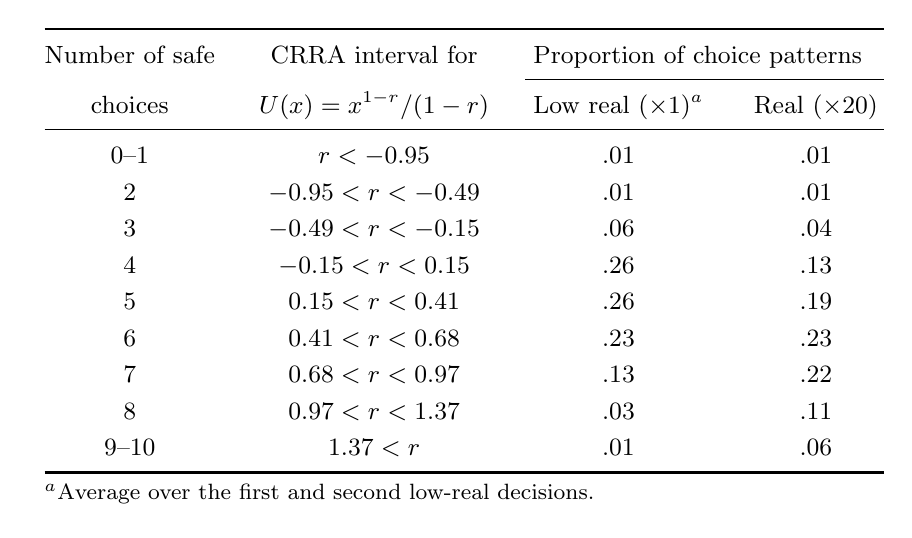
\begin{tikzpicture}
  \node[inner sep=0pt] {
    \small
    \renewcommand{\arraystretch}{1.20}
    \setlength{\tabcolsep}{8pt}
    \begin{tabular}{@{}c c cc@{}}
      \toprule
      Number of safe & CRRA interval for & \multicolumn{2}{c}{Proportion of choice patterns} \\
      \cmidrule(l){3-4}
      choices & $U(x)=x^{1-r}/(1-r)$ & Low real ($\times1$)$^{a}$ & Real ($\times20$) \\
      \midrule
      0--1  & $r<-0.95$           & .01 & .01 \\
      2     & $-0.95<r<-0.49$     & .01 & .01 \\
      3     & $-0.49<r<-0.15$     & .06 & .04 \\
      4     & $-0.15<r<0.15$      & .26 & .13 \\
      5     & $0.15<r<0.41$       & .26 & .19 \\
      6     & $0.41<r<0.68$       & .23 & .23 \\
      7     & $0.68<r<0.97$       & .13 & .22 \\
      8     & $0.97<r<1.37$       & .03 & .11 \\
      9--10 & $1.37<r$            & .01 & .06 \\
      \bottomrule
      \multicolumn{4}{@{}l@{}}{\footnotesize $^{a}$Average over the first and second low-real decisions.} \\
    \end{tabular}
  };
\end{tikzpicture}
\end{document}
